\begin{savequote}
Apparently the child recognizes speech sounds as patterns of gestures.
\qauthor{Israel Rosenfield, \textit{The invention of memory}}
\end{savequote}
\chapter{Unified Gesture Recognition Framework}

As mentioned in the Chapter~\ref{chap:related} Related Work, most prior works
focus on recognizing one form of gestures: either path or pose gestures.
We could conceivably just combine the two forms by first deciding what
category the gesture is and then apply different recognition methods. However making
decisions too early may not be robust. For example, if the system categorizes
the gestures wrongly, it will be hard to correct that in the later stage. We
could also apply two different methods simultaneously, e.g., compute likelihood
from HMMs for path gestures and compute SVM probability scores for pose
gestures, but it is not clear how these probabilities can be compared for making
final decisions.

As a result, I developed a unified probabilistic framework to handle the two
forms of gestures so that probabilities are comparable. During online
recognition, the system makes soft decisions rather than hard decisions, and
propagates probabilities until a response (decision)
from the system is required according to the flow of the currently most likely
gesture.
This chapter gives details about this unified framework.

\section{Gesture Modeling using Hierarchical HMM}
In Section~\ref{sec:temporal-model}, I explained that
a gesture consists of three phases: \textit{pre-stroke}, \textit{nucleus}, and \textit{post-stroke}. 
This temporal model can be represented by a stochastic state
machine (the first level in Figure~\ref{fig:hhmm}).
Each gesture phase includes a sequence of hand/arm movement which can 
also be represented by a stochastic state machine (the second level in the figure), with each state generating an
observation (i.e., the feature vector).
This process can be viewed as a hierarchical HMM (HHMM). We can combine gestures
together to form another stochastic state machine (Figure~\ref{fig:combined}).

\begin{figure}[tbh]
\centering
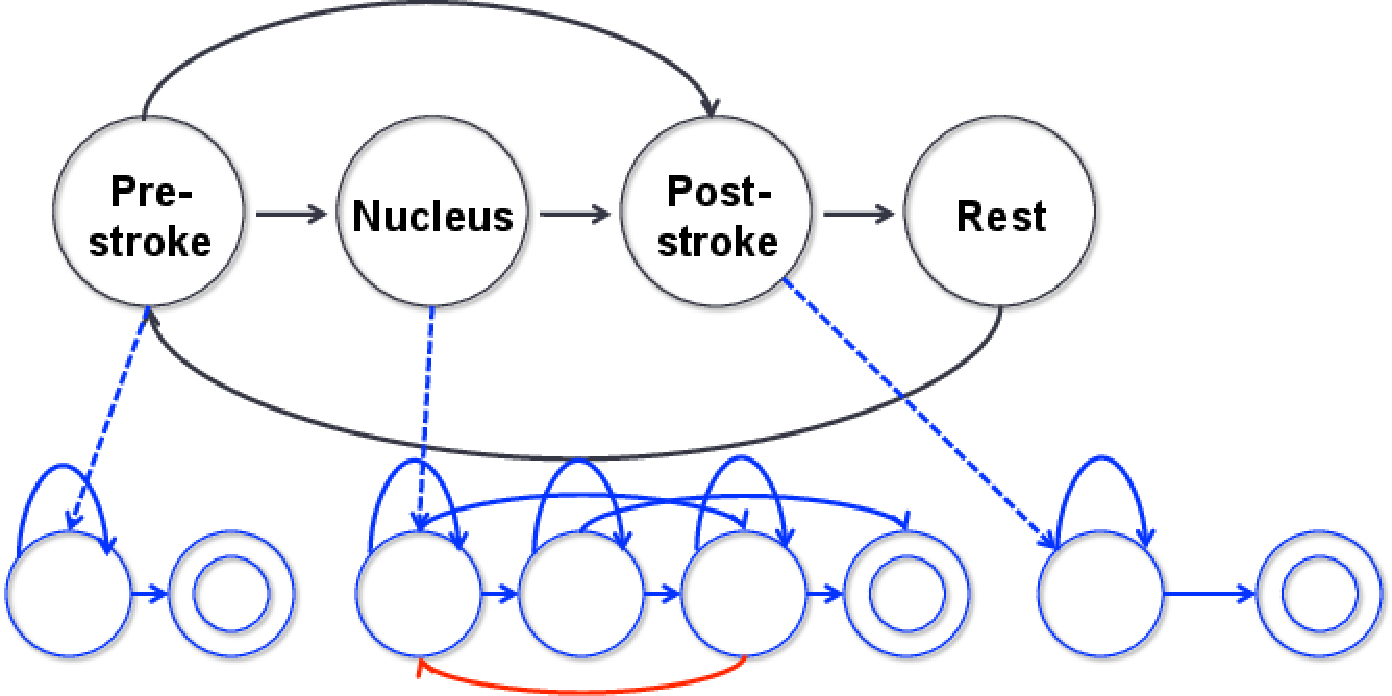
\includegraphics[clip, width=0.7\columnwidth]{figures/hhmm.pdf}
\caption{State transition diagram of the HHMM representation of gesture phases.
Solid arcs represent horizontal transitions between states; dotted arcs
represent vertical transition, i.e., calling a sub-HMM. Double-ringed states
are end states.}
\label{fig:hhmm}
\end{figure}

\begin{figure}[tbh]
\centering
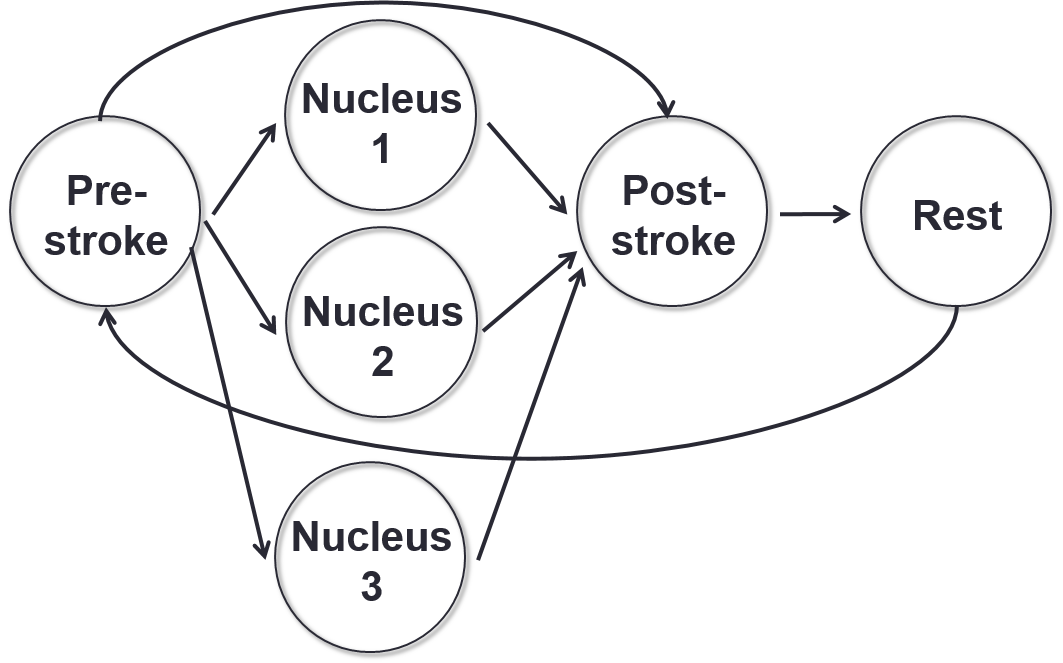
\includegraphics[width=0.7\columnwidth]{figures/combined.png}
\caption{Stochastic state machine for all gestures. The
hidden states for pre-stroke and post-stroke phases are shared among all the
gestures.
}
\label{fig:combined}
\end{figure}

The HHMM is an extension of the HMM that is designed to model domains with
hierarchical structure and/or dependencies at multiple length/time
scales~\cite{murphy02}. In an HHMM, the states of the stochastic automaton can
emit single observations or strings of observations. Those that emit single
observations are called ``production states'' (blue circles in
Figure~\ref{fig:hhmm}, and those that emit strings are termed ``abstract
state'' (black circles). 

We can represent the HHMM as a dynamic Bayesian network\footnote{See
Appendix~\ref{app:dbn} for more details about DBN.} (DBN)~\cite{murphy02} as
shown in Figure~\ref{fig:ahmm}.
The state of the whole HHMM at time $t$ is encoded by the vector $(G_t, P_t, S_t)$ where $G_t$ is the gesture label, $P_t$ is the
phase label, and $S_t$ is the hidden state representing a sub-stage in a
gesture phase. $F_t^d$ is a binary indicator variable that is
``on'' (has value 1) if the lower level HMM at time $t$ has just ``finished''
(i.e., is about to enter an end state), otherwise it is ``off'' (has value 0).
The bottom level $X_t$ are the observations. 

The $F_t^d$ binary indicator in the hierarchical model allows us to do
simultaneous segmentation and recognition. I want to avoid doing segmentation first and then find the most
likely HMM for the given sequence, because segmentation based on
differentiating rest position versus non-rest position will not allow the system
to respond fast enough. I want the system to respond at the beginning of the
post-stroke phase rather then at the beginning of the rest position. In
addition, making a hard decision on segmentation can introduce errors that
are hard to correct later. 

Even though the HHMM gives an appropriate modeling of temporal gestures,
performing exact inference on it can be slow due to the loops in the graphical
model. In the real-time system, I flatten the hierarchical HMM into a one-level
HMM for fast training and inference by creating an HMM state for
every leaf in the HHMM state transition diagram \cite{murphy02}, assuming that
the states in the sub-HMMs are not shared. The effect of The $F_t^d$ binary
indicator can be achieved by modeling the termination probability of each
state, $t(\text{END}|s)$, i.e., the probability for state $s$ to transit to the
end state in the sub-HMM.
This conversion is always done in speech recognition as well for speed and ease of processing.

\tikzstyle{vertex}=[circle, draw, minimum size=16pt, inner sep=0pt]
\tikzstyle{observed-vertex}=[circle, draw, minimum size=16pt, inner sep=0pt,
               fill=black!20] 
\tikzstyle{edge} = [draw, thick, -]
\tikzstyle{directed-edge} = [draw, thick, ->]

\begin{figure}[tbh]
\centering
  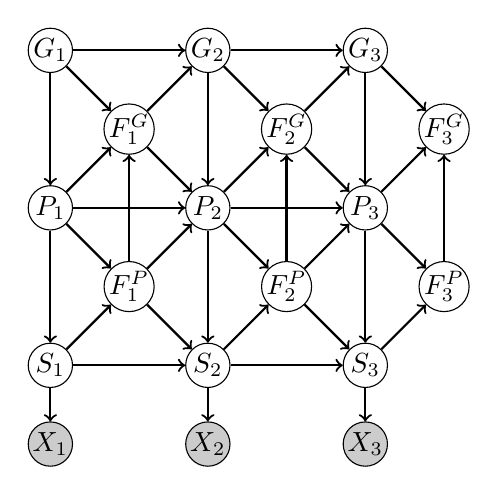
\begin{tikzpicture}[auto,swap, scale=2]
    % First we draw the vertices
    \foreach \pos/\name in {{(0, 2)/P_1}, {(1, 2)/P_2}, {(2,2)/P_3},
      {(0, 3)/G_1}, {(1, 3)/G_2}, {(2,3)/G_3},     
      {(0.5,2.5)/F_1^G}, {(1.5,2.5)/F_2^G}, {(2.5, 2.5)/F_3^G},
      {(0.5,1.5)/F_1^P}, {(1.5,1.5)/F_2^P}, {(2.5, 1.5)/F_3^P}, {(0, 1)/S_1},
      {(1, 1)/S_2}, {(2, 1)/S_3}} 
      \node[vertex] (\name) at \pos {$\name$};
    \foreach \pos/\name in {{(0, 0.5)/X_1}, {(1, 0.5)/X_2}, {(2, 0.5)/X_3}}
      \node[observed-vertex] (\name) at \pos {$\name$};
    % Connect vertices with edges and draw weights
    \foreach \source/ \dest in {P_1/S_1, S_1/X_1, P_1/F_1^P, S_1/F_1^P,
        G_1/P_1, G_2/P_2, G_3/P_3, G_1/G_2, G_2/G_3,
        G_1/F_1^G, G_2/F_2^G, G_3/F_3^G, P_1/F_1^G, P_2/F_2^G, P_3/F_3^G,
        F_1^G/G_2,  F_2^G/G_3, F_1^G/P_2, F_2^G/P_3, 
        F_1^P/F_1^G, F_2^P/F_2^G, F_3^P/F_3^G, 
        F_1^P/P_2, P_1/P_2, P_2/S_2, S_2/X_2, P_2/F_2^P,
        S_2/F_2^P, F_2^P/P_3, P_2/P_3, P_3/S_3, S_3/X_3,
        P_3/F_3^P, S_3/F_3^P, S_1/S_2, S_2/S_3,
        F_1^P/S_2, F_2^P/S_3} 
      \path[directed-edge] (\source) -- (\dest);
  \end{tikzpicture}
  \caption{DBN representation of the HHMM for the temporal gesture model. $G_t$ is the gesture label, $P_t$ is the
phase label, and $S_t$ is the hidden state representing a sub-stage in a
gesture phase. $F_t^d = 1$ if the HMM at the lower level has finished
(entered its exit state), otherwise $F_t^d = 0$. Shaded nodes are observed; the
remaining nodes are hidden.}
  \label{fig:ahmm}
\end{figure}

\section{Unified Framework}
I flatten the HHMM into a single level HMM with discrete hidden states 
representing sub-stages of gesture phases. The assumption is that
gesture phases of different gestures do not share sub-stage hidden states.

Based on the standard HMM\footnote{See Appendix~\ref{app:hmm} for more details
about HMM.} formulation, the probability of a sequence of observation, $\underline{x}_{1:T} = \underline{x}_1\ldots\underline{x}_T$, and
the corresponding hidden states sequence, $s_{1:T} = s_1\ldots s_T$, is given by
\begin{align}
P(\underline{x}_{1:T}, s_{1:T};\underline{\theta}) = 
    t(s_1)t(\text{END}|s_T)\prod_{t = 2}^T t(s_t | s_{t-1})\prod_{t = 1}^T
    e(\underline{x}_t|s_t)\label{eq:hmm}
\end{align}
where $\underline{\theta}$ represents the model parameter vector which includes
the initial state probabilities $t(s)$, the state transition probabilities $t(s'|s)$, the 
emission probabilities $e(\underline{x}|s)$,
and the termination probabilities $t(\text{END}|s)$ for $s, s'\in \{1, 2,\ldots
k\}$. In this section, I describe how I model these conditional
probability distributions (CPDs), and compute the model parameters for both
path and pose gestures, combining them together under the unified HMM-based
framework. Note that the term ``unified framework'' means that the two forms of
gestures are combined under the same probabilistic framework, but there are
still differences in the models for the two gestures, e.g., different topologies
and different training strategies.

\subsection{Path Gestures}
If we have ground truth labels for the pre-stroke, the nucleus and the
post-stroke phases as in the ChAirGest dataset, we can train the sub-HMMs for
each phase and each gesture separately and then concatenate them (i.e., the
concatenated HMMs\footnote{See my previous publication~\cite{yin13} for
details.}).
However in practice, for example if we want users to be able to easily add their new gestures by giving a few
examples, it will be tedious to manually label the start and the end of the
three phases. In this case, I use embedded training \cite{young1994}, i.e.
train each phase sub-HMM embedded in an entire gesture segment
(Figure~\ref{fig:embed}).

\begin{figure}[tbh]
\centering
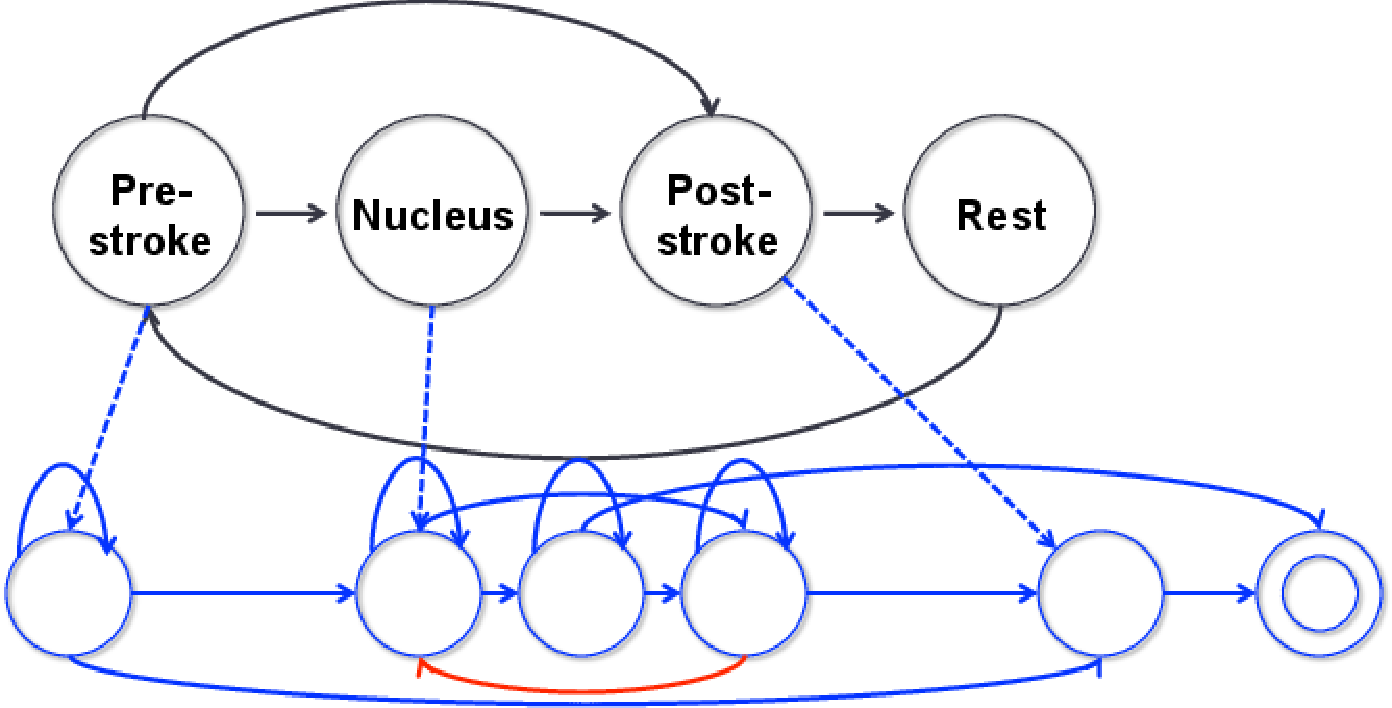
\includegraphics[width=0.7\columnwidth]{figures/embedded.pdf}
\caption{Embedding phase HMMs into an entire gesture.}
\label{fig:embed}
\end{figure}

With the YANG dataset, I choose to use one hidden state for pre-stroke and
post-stroke phases through cross-validation. I use the Bakis (left-right)
model~\cite{Bauer00} for the nucleus phase, but add a backward transition from the last hidden state to the first
one for gestures with an arbitrary number of repetitions (e.g., ``Wave''
gesture) (Figure~\ref{fig:bakis}). 

\tikzstyle{vertex}=[circle, draw, minimum size=16pt, inner sep=0pt]
\tikzstyle{observed-vertex}=[circle, draw, minimum size=16pt, inner
sep=0pt, fill=black!20] 
\tikzstyle{edge} = [draw, thick, -]
\tikzstyle{directed-edge} = [draw, ->]
\begin{figure}[tbh]
\centering
  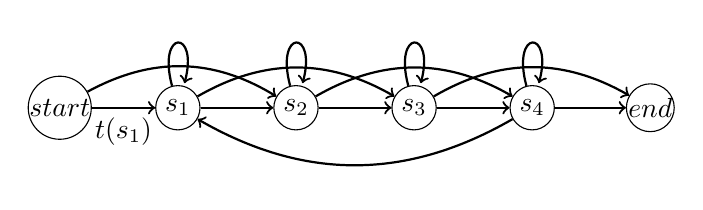
\begin{tikzpicture}[auto,swap, scale=1.5]
    % First we draw the vertices
    \foreach \pos/\name in {{(0, 0)/start}, {(1, 0)/s_1}, {(2, 0)/s_2},
    {(3, 0)/s_3}, {(4, 0)/s_4}, {(5, 0)/end}}
      \node[vertex] (\name) at \pos {$\name$};
    % Connect vertices with edges and draw weights
    \foreach \source/ \dest in {s_2/s_3, s_3/s_4, s_4/end,
    s_1/s_2} \path[directed-edge] (\source) -- (\dest);
    
    \foreach \source/ \dest in {s_1/s_3, start/s_2, s_2/s_4, s_3/end, s_4/s_1} 
      \path[directed-edge] (\source) edge [bend left] (\dest);
      
    \foreach \source/ \dest in {s_1/s_1, s_2/s_2, s_3/s_3, s_4/s_4} 
      \path[directed-edge] (\source) edge [loop above] (\dest);
    
    \path[directed-edge] (start) edge node [below] {$t(s_1)$} (s_1);
  \end{tikzpicture}
  \caption{A state transition diagram of a modified 4-state Bakis model for the nucleus phase.}
  \label{fig:bakis}
\end{figure}

In Chapter~\ref{chap:feature}, I showed that the features I use follow mixture
of Gaussians (MoG) distributions, hence I use MoG with diagonal covariances to
model the emission probability, i.e.,
\begin{align}
e(\underline{x} | s) = \sum_{m=1}^k q(m | s)\mathcal{N}(\underline{x};
\mu_{s,m}, \Sigma_{s, m})
\end{align}
where $k$ is the number of mixtures.
Figure~\ref{fig:mog} shows the DBN representation of an HMM of MoG emission
probabilities. The covariance, $\Sigma_{s, m}$, has a fixed prior of $0.01\times
I$ which is added to the maximum likelihood estimate to prevent the covariance from shrinking to a point/delta function. 

\begin{figure}[tbh]
\centering
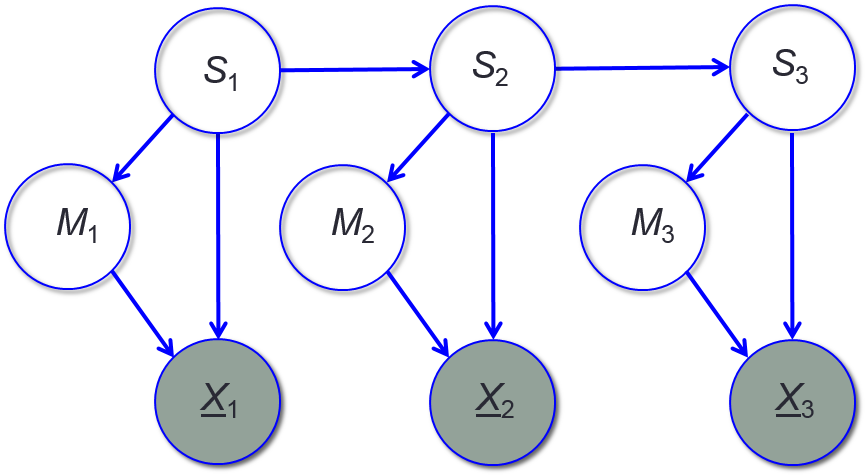
\includegraphics[width=0.5\columnwidth]{figures/mog.png}
\caption{DBN representation of HMM with mixture of
Gaussians emission probabilities.}
\label{fig:mog}
\end{figure}

\subsubsection{Training Strategies}
I use a two-pass training to estimate the model parameters for each path
gesture HMM separately. Currently, training is done in MATLAB using Kevin
Murphy's HMM toolbox\footnote{\url{https://code.google.com/p/bnt/}}.

The first pass is Viterbi training. In this pass, only the first state
(i.e., the pre-stroke hidden state) can be the initial state and the last state
(i.e., the post-stroke hidden state) can be the termination state. The emission
probability parameters are initialized by uniformly segmenting the data and
associating each successive segment with successive states~\cite{young1994}. For
each segment, the K-means algorithm is used to initialize MoG parameters. The
Viterbi training provides a better alignment of data with the hidden states, and
thus gives a better initialization of the MoG parameters.

The second pass is Baum-Welch training that computes the maximum likelihood
estimate of the parameters.
It uses the estimated MoG parameters as the initial values. It also relaxes the
initial state probabilities (allowing the first two states to be the start
state) and the termination probabilities (allowing the last two states to be the
termination state). This allows the possibility of transitions between nucleus
phases without going through pre-strokes and post-strokes when we combine the
individual gesture HMMs together. For natural interaction, this is important
because sometimes users may do a gesture immediately after another. When
initializing the transition matrix, all the allowed transitions are set to the same value, so that no states are favored arbitrarily. Transitions that are not allowed are initialized to zero.

The Baum-Welch estimation formulae for MoG parameters and transition parameters
are well established. Here, I give the formula for the termination probability.
Given $N$ training sequences, the update for the termination probability during the $i$th iteration is 
\begin{displaymath}
t^i(\text{END}|s) = \frac{\sum_{j = 1}^N \overline{count}(j, s\rightarrow
END;\underline{\theta}^{i-1})} {\sum_{j = 1}^N\sum_{s'} \overline{count}(j, s\rightarrow s';\underline{\theta}^{i-1})}
\end{displaymath}
where $\overline{count}(j, s\rightarrow END;\underline{\theta}^{i-1})$ is the expected count of 
$s$ being the end state. We can use the usual forward-backward algorithm to compute all the 
expected sufficient statistics by adding a dummy END state to the end of each
sequence (see Appendix~\ref{sec:term} for details).

\subsection{Pose Gestures}
I use one hidden state to represent pose gestures. Let
$s_{\text{pose}}$ be the single hidden state for the nucleus phase of a
pose gesture (Figure~\ref{fig:single}). Within a user,
there may be variation in the hand pose for a gesture with distinct hand pose.
For example, the Point hand pose can have different orientations.
Hence, I also use the MoG for the emission probability
$e(\underline{x} | s_\text{pose})$. 

\begin{figure}[tbh]
\centering
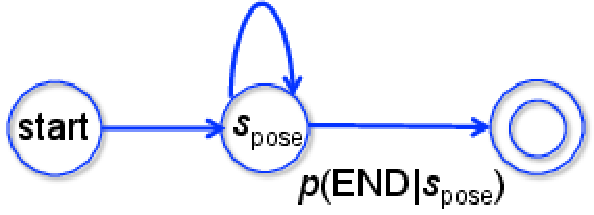
\includegraphics[width=0.5\columnwidth]{figures/single_state.pdf}
\caption{State transition diagram of a single state HMM for gestures with
distinct hand poses. }
\label{fig:single}
\end{figure}

The number of mixtures for pose gestures are greater than that of path
gestures however, and they can be different for different pose gestures. This is
because some hand poses may have more variation than others.
For example, the Point gesture may have more variations in orientations than
Grab gesture (hand in fist).

\subsubsection{Training Strategies}\label{sec:pose-gesture}
Instead of doing embedded
training, I directly compute the maximum likelihood estimates of the MoG
parameters for emission probability of $s_{\text{pose}}$ because there is only
on hidden state.

The number of mixtures is
determined using Bayesian Information Criterion (BIC)~\cite{fraley06}:
\begin{align*}
\text{BIC}\eqdef2\text{loglik}(\underline{x}_{1:n}, \underline{\theta}_k^*) -
(\text{\# params})\log(n)
\end{align*}
where $\text{loglik}(\underline{x}_{1:n}, \underline{\theta}_k^*)$ is the
maximized loglikelihood for the data and the model with $k$ mixtures per state, (\# params) is the number of independent parameters to be estimated in the model, and $n$ is the number of observations in
the data. Let $d$ be the feature vector dimension, then $\mu_{s,m}$ for
hidden state $s$ and mixture $m$ has $d$ independent parameters, and the
diagonal covariance matrix $\Sigma_{s,m}$ has $d$ independent parameters as
well. Because $\sum_{m=1}^k q(m | s) = 1$, the number of independent parameters
for the weights $q(m|s)$ is $k - 1$. Hence,(\# params) is computed as:
\begin{align*}
\text{\# params} = (k - 1) + (d + d) * k
\end{align*}
The $k$ that gives the highest BIC is chosen from a predetermined range.

For each $k$, Expectation Maximization (EM) is used to estimate the means,
covariance matrices and mixture probabilities of the MoG. As the EM algorithm may
converge to a local optimum of the observed data likelihood~\cite{dicintio12}, I
repeat the optimization 3 times using K-means algorithm with random
initialization to set the initial cluster centers, and choose the model that
gives the maximum likelihood.

The training data for pose gestures should contain random variations in the
hand movement so that the resultant variances for the motion features will be
larger, making motion features less important in
$e(\underline{x}|s_{\text{pose}})$. In Figure~\ref{fig:covariance}, I compare
two covariance matrices of MoG for hidden states from two forms of gestures. The
variance values are normalized between the two matrices for each feature to make
them comparable. We can see that the variances for the motion features (features
1--9) are larger for the pose gesture.

\begin{figure}[tbh]
\centering
\subfigure[Hidden state of a path gesture.]{
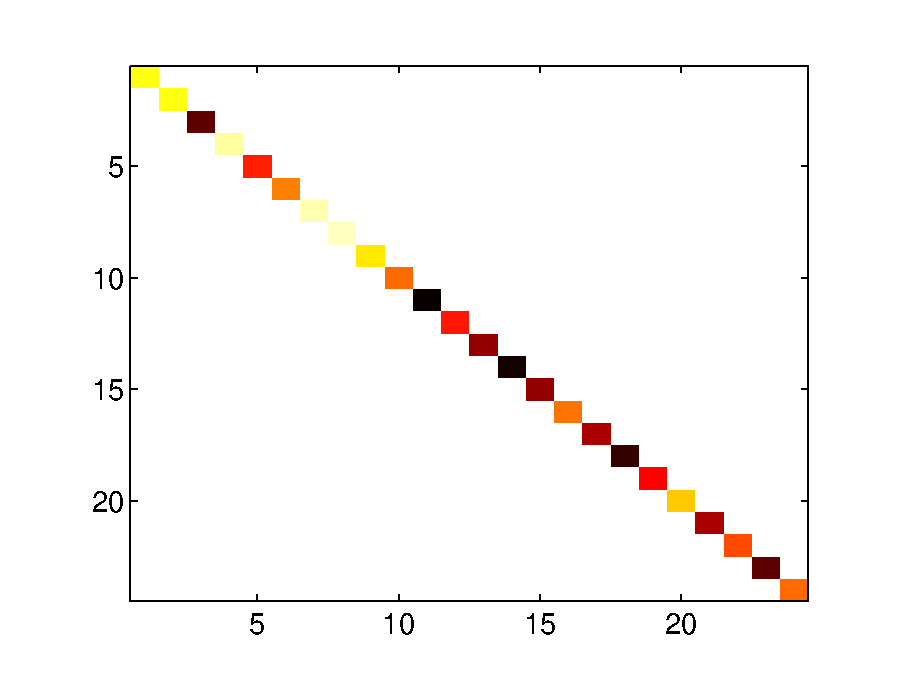
\includegraphics[trim=1.3cm 0 1cm
0.5cm, clip, width=0.45\columnwidth]{figures/covariance_path.eps} }
\subfigure[hidden state of a pose gesture.]{
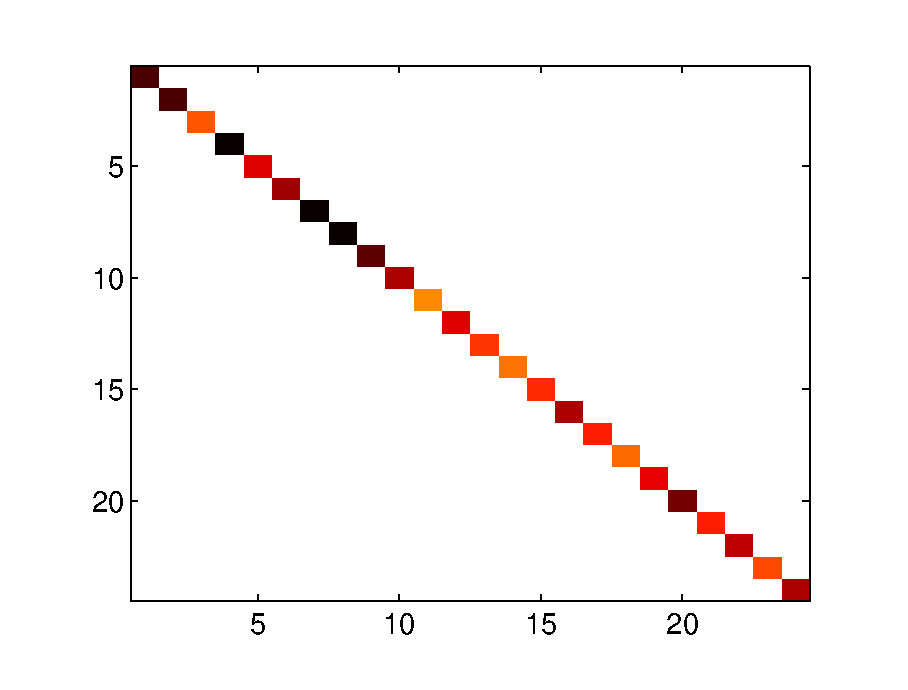
\includegraphics[trim=1.3cm 0
1cm 0.5cm, clip, width=0.45\columnwidth]{figures/covariance_pose.eps} }
\caption{Visualization of normalized covariance matrices of MoG for different
hidden states. The darker the color, the larger the variance.}
\label{fig:covariance}
\end{figure}

It is possible that a gesture with a distinct path also has the same hand pose
as another gesture with distinct hand pose, for instance, some user may prefer
to do the Circle gesture with a point hand pose. In this case, the gesture
will be recognized as the Circle gesture because it matches both the hand
pose and the path and thus the Circle gesture would have a higher likelihood
after considering a few consecutive frames.

Since there is only one hidden state for $s_{\text{pose}}$, its transition
probability is 1. Its termination probability is estimated according to the
expected duration of the gesture. The self-arc on a state in an HMM defines a 
geometric distribution over waiting time \cite{murphy02}. In the case of a
single state HMM, the probability of remaining in state $s_{\text{pose}}$ for
exactly $d$ steps is $P(d) = p(1-p)^{d - 1}$, where $p = P(END|s_\text{pose})$
is the termination probability for $s_{\text{pose}}$. This means the expected
number of steps remaining in state $s_{\text{pose}}$ is $\frac{1}{p}$. I assume
that the minimum duration of a path gesture is one
second (30 frames). The termination probability $P(END|s_\text{pose})$ is then set to
be less than $\frac{1}{30}$.

I also use one hidden state to model the rest position in a similar way.

\section{Real-time Gesture Recognition}
I train one HMM, $\underline{\theta}_g$, for each gesture (path or pose) $g\in
\{1\ldots G\}$, then combine them into a one-level flattened HMM, assuming uniform transition probabilities among gestures.

\subsection{Combined HMM}
I use the superscript $c$ to denote the model
parameters in the combined HMM. Let $K_{g}$ be the number of hidden states for
gesture $g$. The total number of hidden states in the combined HMM, $K^c$, is then
\begin{align*}
K^c = \sum_g K_{g}
\end{align*}
The model for each path gesture starts with a hidden state for the pre-stroke,
then 1 or 2 hidden states for the nucleus, followed by a hidden state for the
post-stroke. Each pose gesture has a hidden state for the nucleus. The combined HMM has a sequential labeling for these models� hidden states,
with the hidden state label for the pre-stroke of the second gesture model following
the hidden state label for post-stroke of the previous gesture, etc.
Formally, the new hidden states labels are in $\{1\ldots K^c\}$, and
the hidden states from $(\text{base}_i + 1)$ to $(\text{base}_g + K_{g})$
belongs to gesture $g$ where $base_g$ is the base index
\begin{align*}
\text{base}_g = \sum_{j=1}^{g-1}K_{j}
\end{align*}
Figure~\ref{fig:combined-hmm} gives an example of the labeling scheme in
the combined HMM. This scheme allows me to easily map a hidden state label back
to its corresponding gesture and phase.

\begin{figure}[tbh]
\centering
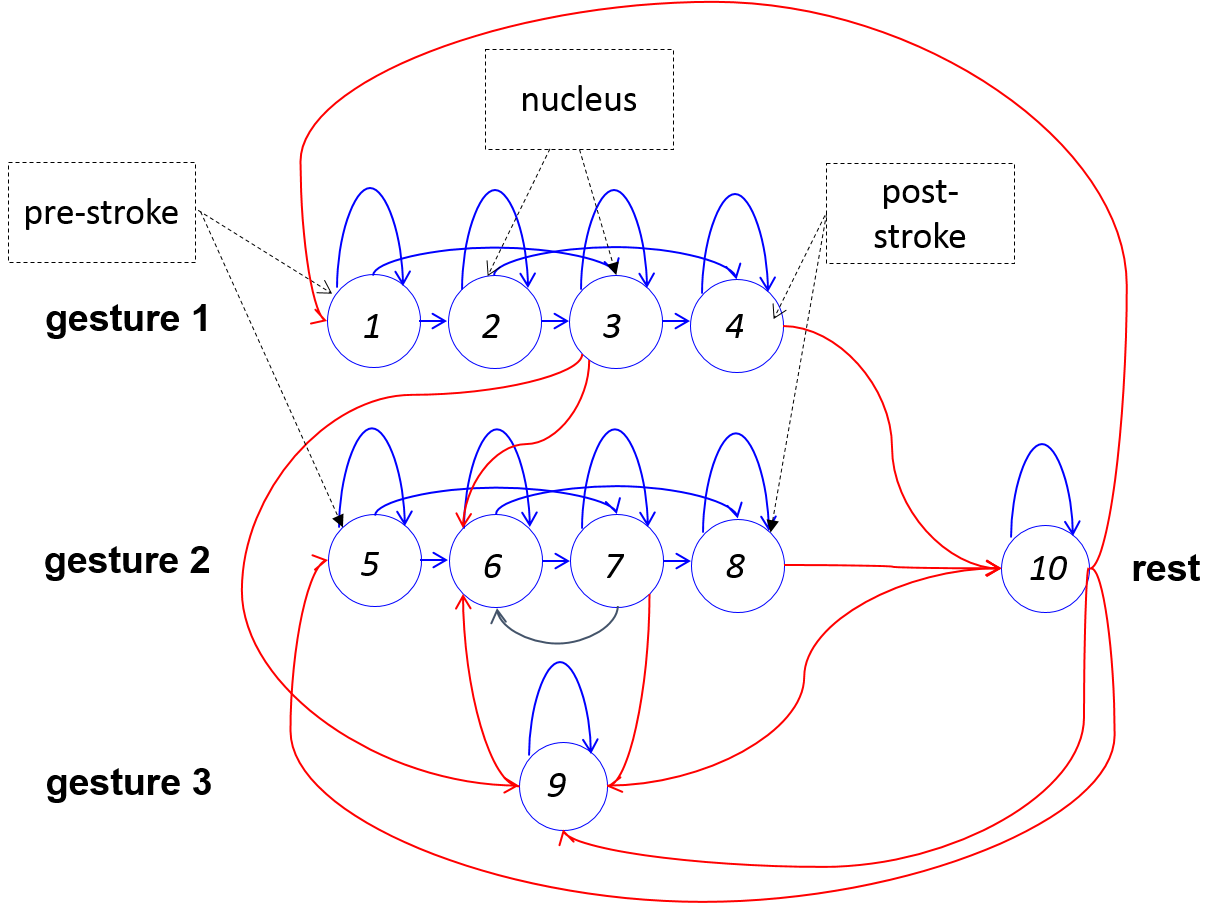
\includegraphics[width=0.9\columnwidth]{figures/combined_hmm.png}
\caption{Combined HMM. The red lines are examples of new transitions. Not all
possible transitions are shown so that the diagram is not cluttered.}
\label{fig:combined-hmm}
\end{figure}

The non-trivial part in creating the combined HMM is computing the new 
transition probabilities. The initial state probability in the combined
HMM, $t^c(s)$, for $s\in\{1\ldots K^c\}$ is
\begin{align*}
t^c(s) = \frac{t(s)}{\sum_{s'=1}^{K^c} t(s')}
\end{align*}
The probability of an $s$ to $s'$ transition
in the combined model is the sum over all paths from $s$ to
$s'$ for $s, s'\in\{1\ldots K^c\}$~\cite{murphy02}. In our model, 
\begin{align}
t^c(s'|s) = t(s' | s) (1-t(\text{END}|s)) +
t(\text{END}|s)t^c(s')
\label{eq:combined-transition}
\end{align}
where $t(s'|s)$ is the transition probability in the individual gesture HMM if
$s$ and $s'$ are from the same gesture; otherwise it is zero. Note that
$t(s'|s)$ is normalized such that $\sum_{s'}t(s'|s) = 1$ without taking into
account the termination probability $t(\text{END}|s)$ (as the end state is not
an actual hidden state), hence it is necessary to multiply $t(s'|s)$ by $
(1-t(\text{END}|s))$ in Equation~\ref{eq:combined-transition} to get the actual
unnormalized probability.

As the pre-strokes and post-strokes for different gestures can be similar, I
allow sharing of the pre-strokes and post-strokes by adding a small probability
(0.01) among pre-stroke hidden states and among post-stroke hidden states.

Finally, we need to make sure that the new transition matrix is stochastic,
i.e., 
\begin{align*}
\sum_{s' = 1}^{K^c} t^c(s'|s) = 1
\end{align*}
by normalizing $t^c(s'|s)$.

\subsection{Online Inference}
Once we have a combined model, I use fixed-lag smoothing \cite{murphy02} to do
online inference on the flattened HMM for real-time gesture recognition.
Fixed-lag smoothing is a modified forward-backward algorithm. Unlike online
filtering, which estimates the belief state at current time $t$ using forward
pass only, we estimate the state at $t - l$, given all the evidence up to the
current time $t$, i.e., compute $\gamma_{t - l}(s) \eqdef P(S_{t -
l} = s|\underline{x}_{1:t})$, where $l > 0$ is the lag. Introducing lag time is
a tradeoff between accuracy and responsiveness. Using some future evidence to
smooth the estimate can increase the accuracy while adding some delay. However
if the delay is small, it might be unnoticeable.
In the Experiment Evaluation section (Section~\ref{sec:evaluation}), we show
details about the relationship between $L$ and the recognition performance.

Fixed-lag smoothing can be implemented efficiently. We compute forward
probabilities $\alpha_t(s) \eqdef P(S_t = s|\underline{x}_{1:t})$
normally\footnote{It is more common (see e.g.,~\cite{Rabiner90}) to define
$\alpha_t(s) = P(S_t = s, \underline{x}_{1:t})$; the difference is discussed in
Section~\ref{sec:hmm-infernece}.} and keep a history window of
$\alpha_{t - l}\ldots\alpha_t$.
At every time frame, we compute backward probabilities $\beta_{t-l}(s)\eqdef
P(\underline{x}_{t-l+1:t}|S_{t-l}=s)$ from current time $t$ to $t - l$, i.e.,
form $l=0$ to $l$.
Then we can compute
\begin{align}
\gamma_{t - l} = \alpha_{t - l} \cdot \beta_{t - l}
\end{align}  
The time complexity at each time frame is $O((K^c)^2l)$. Note that at time $t$,
the belief state at $t - l$ is committed, while the belief state from $t - l + 1$ to $t$
will still be revised later.

We can then compute the most likely hidden state at $t - l$:
\begin{align}
\hat{s} = \arg\max_s \gamma_{t - l}(s)
\end{align}
We map the most likely hidden state to the gesture label it
belongs to (including the rest position) and the gesture phase. 

Gesture events are detected at the boundary of a phase change: start pre-stroke,
start gesture nucleus and start post-stroke. In this way
we achieve simultaneous segmentation and recognition. The gesture event
information, together with the gesture label for the nucleus phase, are sent to the application level.

\begin{figure}[t]
\centering
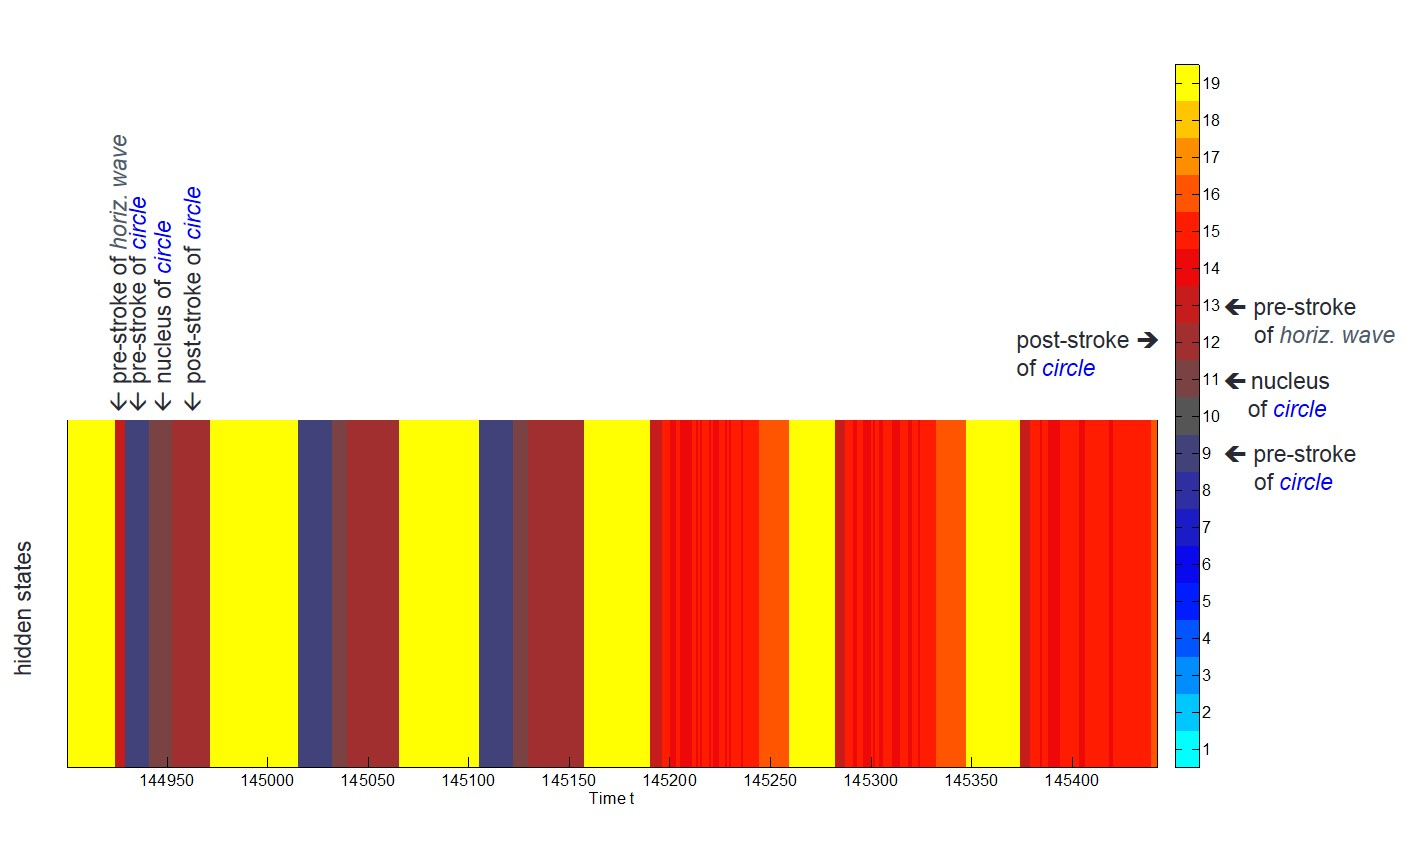
\includegraphics[trim=0 5mm 0
5mm, clip, width=\columnwidth]{figures/hidden_labeled.jpg}
\caption{Most likely hidden states using fixed-lag smoothing. Different colors indicate different hidden states. Yellow indicates rest position.}
\label{fig:visual_hidden}
\end{figure}

Figure~\ref{fig:visual_hidden} shows a visualization of the
most likely hidden states based on online fixed-lag smoothing inference
with $l = 5$ on a test sequence from the YANG dataset.
This is based on an input sequence of 6 gestures. The first 3 gestures are
Circle and the last 3 gestures are Horizontal Wave gestures. Notice that in
the first segment, at the beginning, the most likely hidden state is the
pre-stroke for Horizontal Wave, but since a response is not required at this
time, the wrong estimate does not matter. After a few more frames, the estimates are
updated to have the correct most likely gesture label and the system
responds correctly when it detects the start of the post-stroke of Circle
gesture.

\section{Gesture Spotting}
Identifying gesture phases allows us to distinguish gestures from non-gestures.
As every gesture must have a nucleus, any hand movement that does not have a
nucleus phase can be identified as non-gesture. 

For example, when performing offline recognition on the ChAirGest dataset, I use
MoG models for rest and non-rest positions to find non-rest segments (i.e.,
segments with hand movement) in a test sequence, and for a non-rest segment, use
the Viterbi algorithm to find the most probable hidden state sequence $\hat{s}_1\ldots\hat{s}_T$ using
the mostly likely gesture model $\underline{\theta}_{\hat{g}}$
(see~\cite{yin13} for details).
Again, each hidden state can by classified into a pre-stroke
($s_\text{pre-stroke}$), nucleus ($s_\text{nucleus}$), or post-stroke
($s_\text{post-stroke}$) state.
The start and the end time for a gesture nucleus are the first and the last time
frame $t$ where $\hat{s}_t\in s_{\text{nucleus}}$ respectively. 

\begin{figure}[!tbh]
\centering
\subfigure[Gesture label result.
The pre-stroke and post-stroke phases are indicated by two orange colors (see the color bar).]{
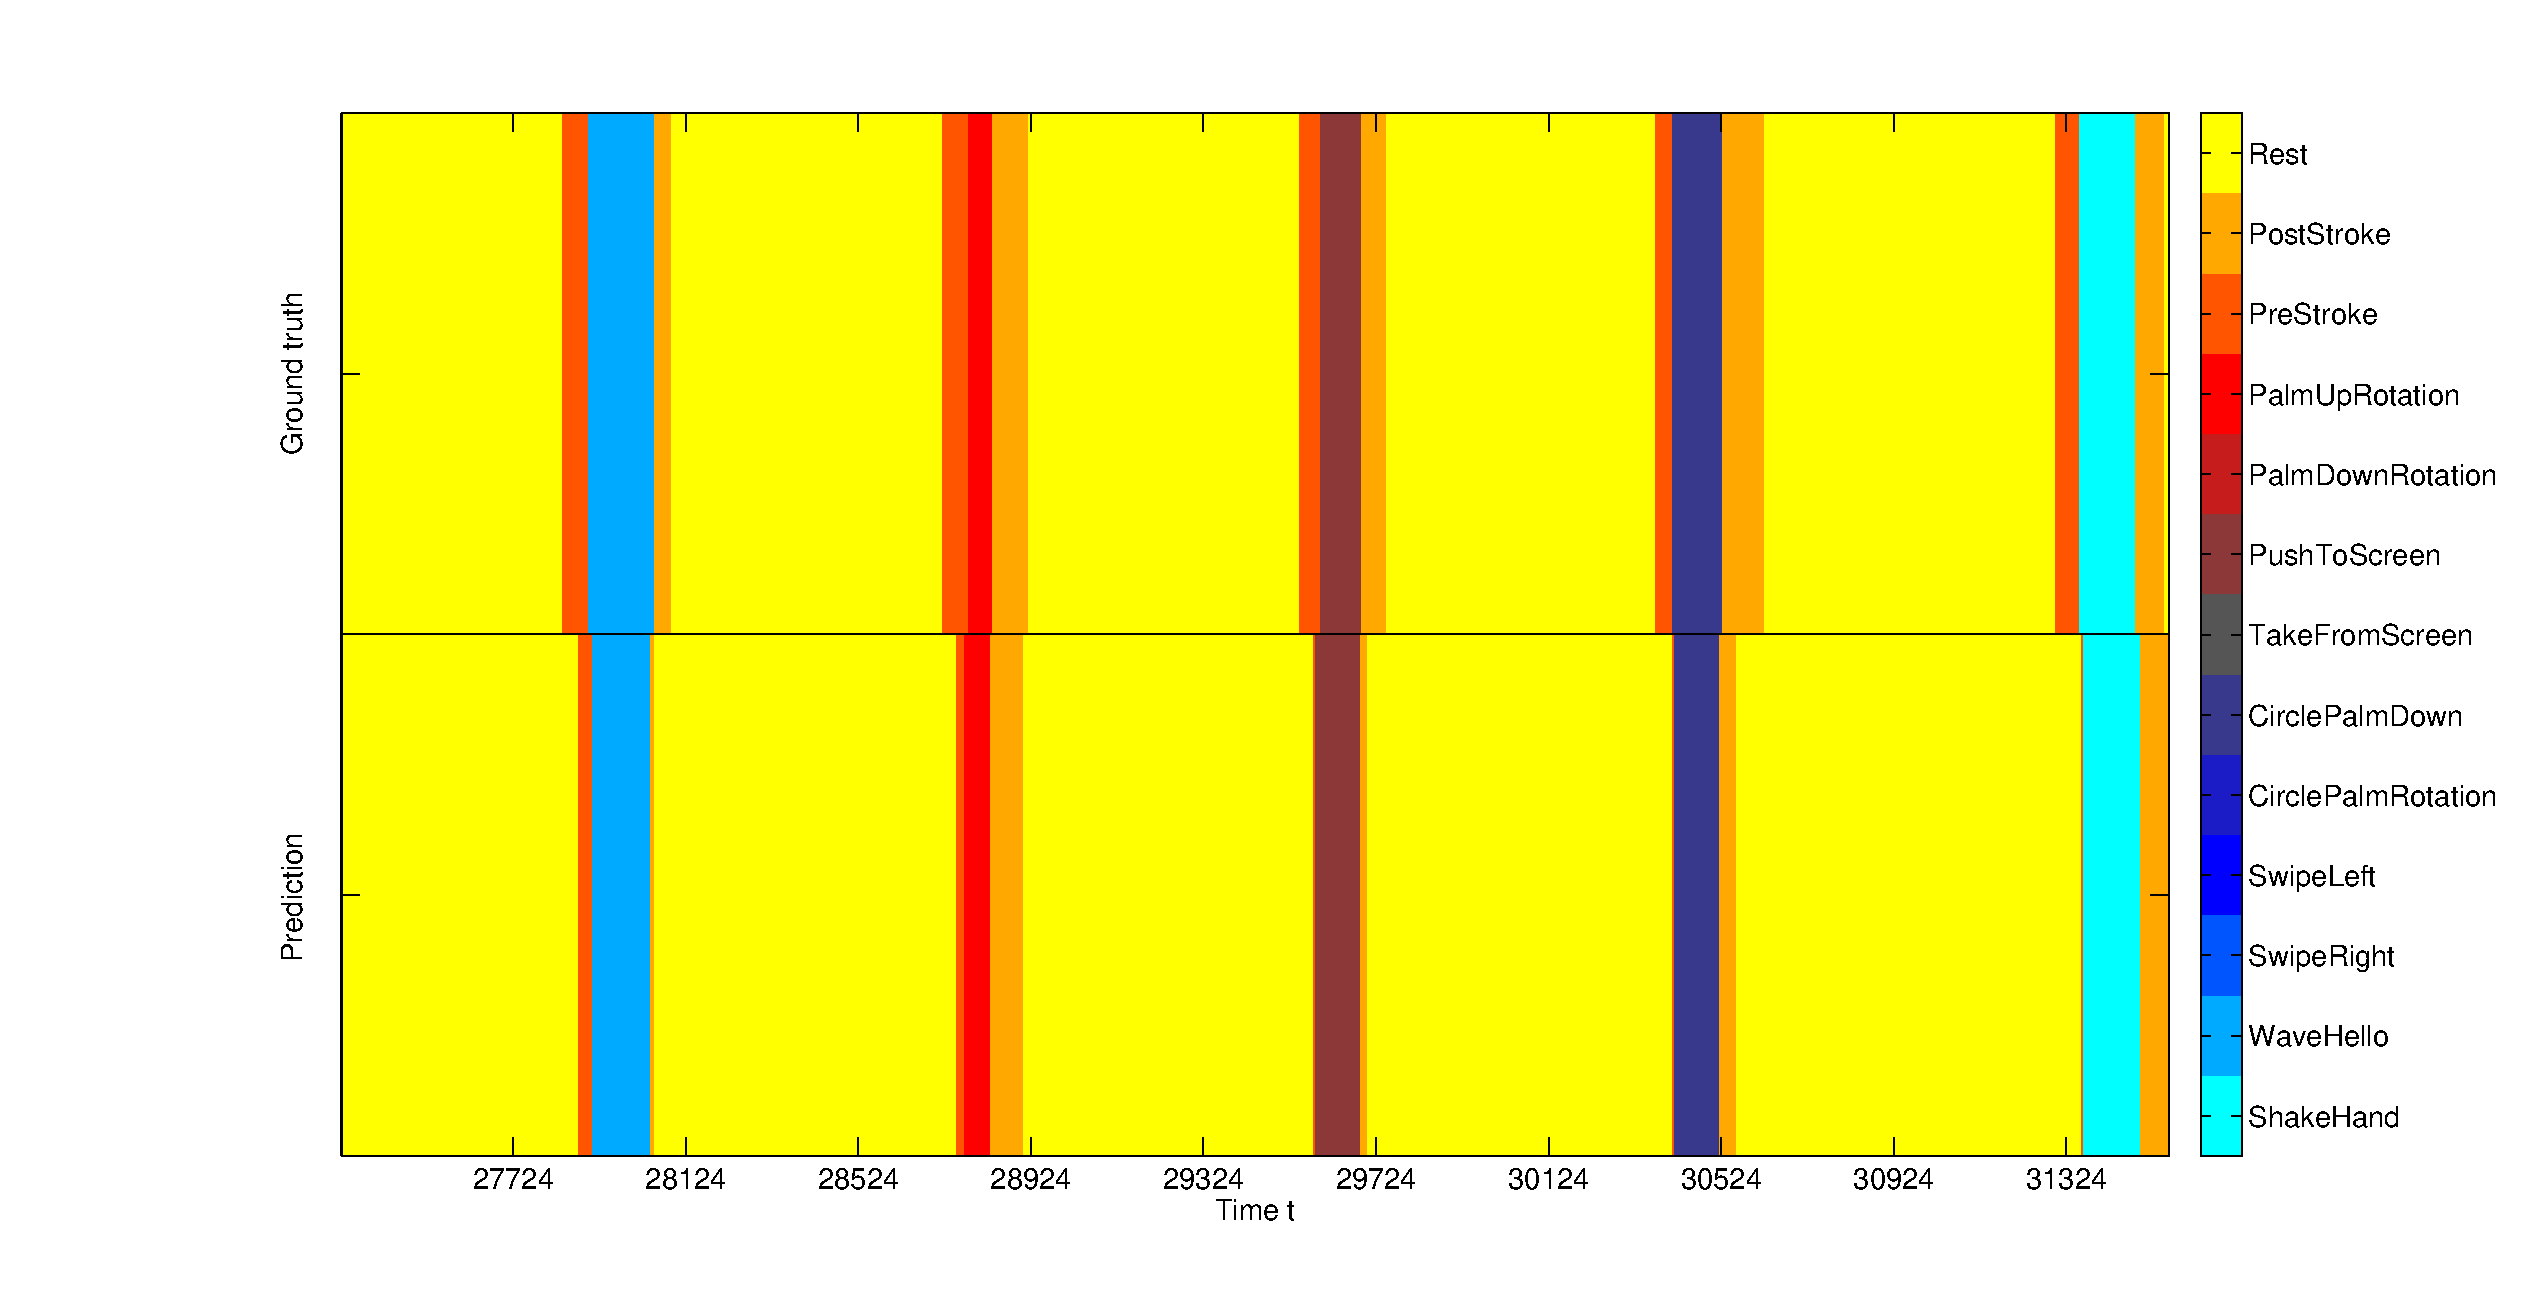
\includegraphics[trim={4cm 1cm 0cm 0.6cm}, clip,
width=1\columnwidth]{figures/gesture.eps}\label{fig:gesture-label}
}
\subfigure[Most probable hidden states.
Colors 1-3 indicate the pre-stroke hidden states, colors 4 - 9
indicate the nucleus hidden states, colors 10 - 12 indicate the post-stroke
hidden states, and color 14 indicates the rest state.]{
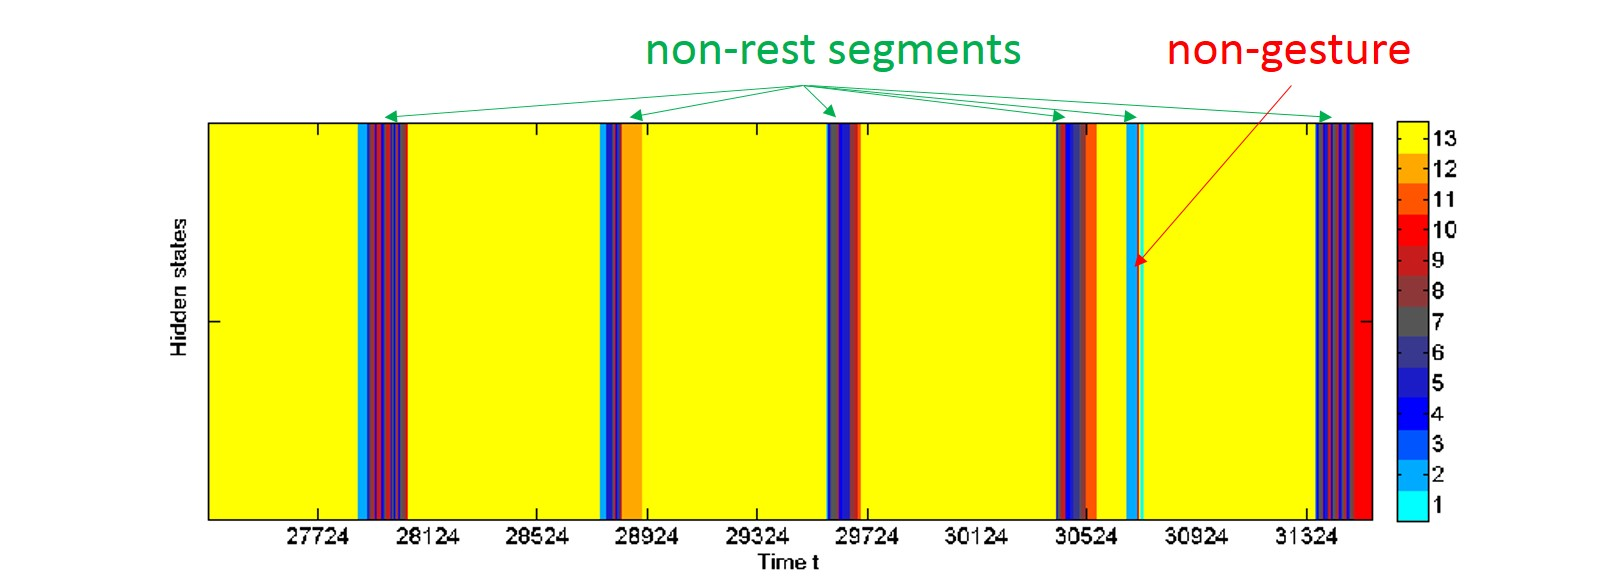
\includegraphics[trim={2.5cm 0cm 0.2cm 0cm}, clip,
width=1\columnwidth]{figures/hiddenstates_labeled.jpg} \label{fig:hiddenstates}
}
\caption{Visualization of gesture recognition result. A non-rest segment
without a nucleus phase (see $t\sim 30700$ in \subref{fig:hiddenstates}) is not
identified as a gesture (no label reported at the same time in
\subref{fig:gesture-label}.}
\end{figure}

Figure~\ref{fig:gesture-label} shows the recognition result visualization for
one test sequence. The first row is the ground truth with different colors
indicating different gesture phases or the rest position.
The second row is my segmentation and recognition result.
Figure~\ref{fig:hiddenstates} shows the color-coded most probable hidden states
for the same sequence.
If a non-rest segment does not contain hidden states belonging to the nucleus
phase, it is ignored (see the blue bar at $t\sim 30700$ in Figure~\ref{fig:hiddenstates}).
In this way, we can spot the actual gestures while filtering out other movements.

Using a thresholding method on the loglikelihood of a
given segment may not be robust because the maximum loglikelihood of a non-gesture
segment among all gesture HMMs can be greater than that of a gesture segment.
The HMM formulation (Equation~\ref{eq:hmm}) implies that the longer the sequence the smaller the
likelihood (and hence the loglikelihood) because there are more probability
terms which are all smaller than 1 in the product terms. For example, the
loglikelihood of the fifth non-rest segment (a non-gesture) in
Figure~\ref{fig:hiddenstates} has a maximum loglikelihood of -296.6, while the
first non-rest segment (a gesture) has a maximum loglikelihood of -785.6. 
Even if we normalize the loglikelihoods by the segment lengths, the normalized
loglikelihood for the non-gesture (-14.8) is still greater than that of the
gesture (-17.9). As non-gestures are often shorter than gesture sequences, it
would hard to set a good threshold.
 
My gesture phase based method can be used in addition to a thresholding method
with a relative conservative threshold, i.e., a threshold that may cause false
positives but no false negatives so that the gesture phase based method can be used to further
filter out false positives.

\section{Concatenated HMM versus LDCRF}
Morency et al. formulated LDCRF~\cite{morency07}, an extension to CRF, and used
it for head and eye gesture recognition. In contrast to HMM which is a
generative model, LDCRF is a discriminative model that gives per frame
classification. It can be used to do simultaneous segmentation and labeling as
well. I applied LDCRF to gesture phase segmentation and recognition, and
compared the result with my concatenated HMM. 

As LDCRF requires per frame labeled training data, we need ground truth labeling
for the gesture phases. Hence, I use the ChAirGest dataset for this
evaluation. For a given non-rest segment,

different hidden states for different pre-stroke and post-stroke phases
for different gestures, increases computation time significantly since it increases quadratically with number of hidden states.
Constrain transition

\begin{table}[tbh]
\centering
\begin{tabular}{|l|l|l|}
\hline
& \thead{LDCRF} & \thead{Concatenated HMMs} \\
\hline
$F_1$ Score & 0.82 (0.03) & \textbf{0.897 (0.03)} \\
\hline
ATSR Score & \textbf{0.923 (0.02)} & 0.907 (0.02) \\
\hline
Final Score & 0.84 (0.02) & \textbf{0.90 (0.02)} \\
\hline
Training Time & 18hr & \textbf{7min} \\
\hline
\end{tabular}
\end{table}